\tikzstyle{vertex}=[circle, draw]
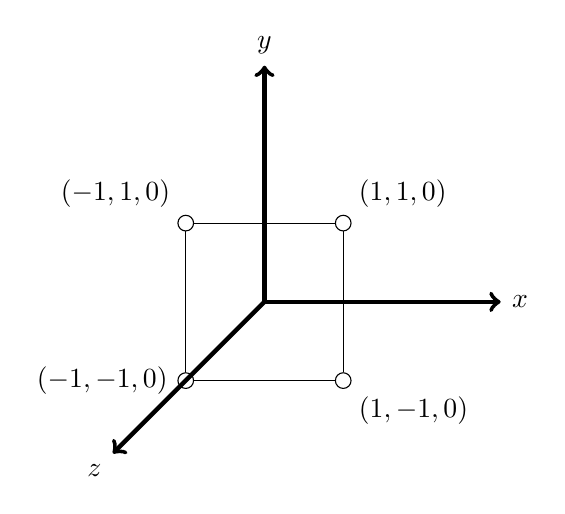
\begin{tikzpicture}[transform shape]
\draw[->,ultra thick] (0,0, 0)--(3,0, 0) node[right]{$x$};
\draw[->,ultra thick] (0,0, 0)--(0,3, 0) node[above]{$y$};
\draw[->,ultra thick] (0,0, 0)--(0,0, 5) node[below left]{$z$};

\node[vertex,inner sep=2pt,minimum size=1pt,label=left:{$(-1, -1, 0)$}](v1) at (-1, -1, 0) {};
\node[vertex,inner sep=2pt,minimum size=1pt,label=below right:{$(1, -1, 0)$}](v2) at (1, -1, 0) {};
\node[vertex,inner sep=2pt,minimum size=1pt,label=above right:{$(1, 1, 0)$}](v3) at (1, 1, 0) {};
\node[vertex,inner sep=2pt,minimum size=1pt,label=above left:{$(-1, 1, 0)$}](v4) at (-1,1, 0) {};

\begin{scope}[every path/.style={-}, every node/.style={inner sep=0pt}]
       \draw (v1) -- node [anchor=south east] {} (v2);
       \draw (v2) -- node [anchor=south west] {} (v3);
       \draw (v3) -- node [anchor=north] {} (v4);
       \draw (v4) -- node [anchor=north] {} (v1);
\end{scope} 
\end{tikzpicture}